\chapter{High dimensional anomaly detection: HPC centers}


\section{Data}

The dataset is a time series with the following fields:
\begin{descriptionlist}
    \item[\texttt{timestamp}] with a $5$ minutes granularity.
    \item[HPC data] technical data related to the cluster.
    \item[\texttt{anomaly}] indicates if there is an anomaly.
\end{descriptionlist}

In practice, the cluster has three operational modes:
\begin{descriptionlist}
    \item[Normal] the frequency is proportional to the workload.
    \item[Power-saving] the frequency is always at the minimum.
    \item[Performance] the frequency is always at the maximum.
\end{descriptionlist}
For this dataset, both power-saving and performance are considered anomalies.


\subsection{High-dimensional data visualization}

\begin{description}
    \item[Individual plots]
        Plot individual columns.

    \item[Statistics]
        Show overall statistics (e.g., \texttt{pandas} \texttt{describe} method)

    \item[Heatmap]
        Heatmap with standardized data.

        \begin{figure}[H]
            \centering
            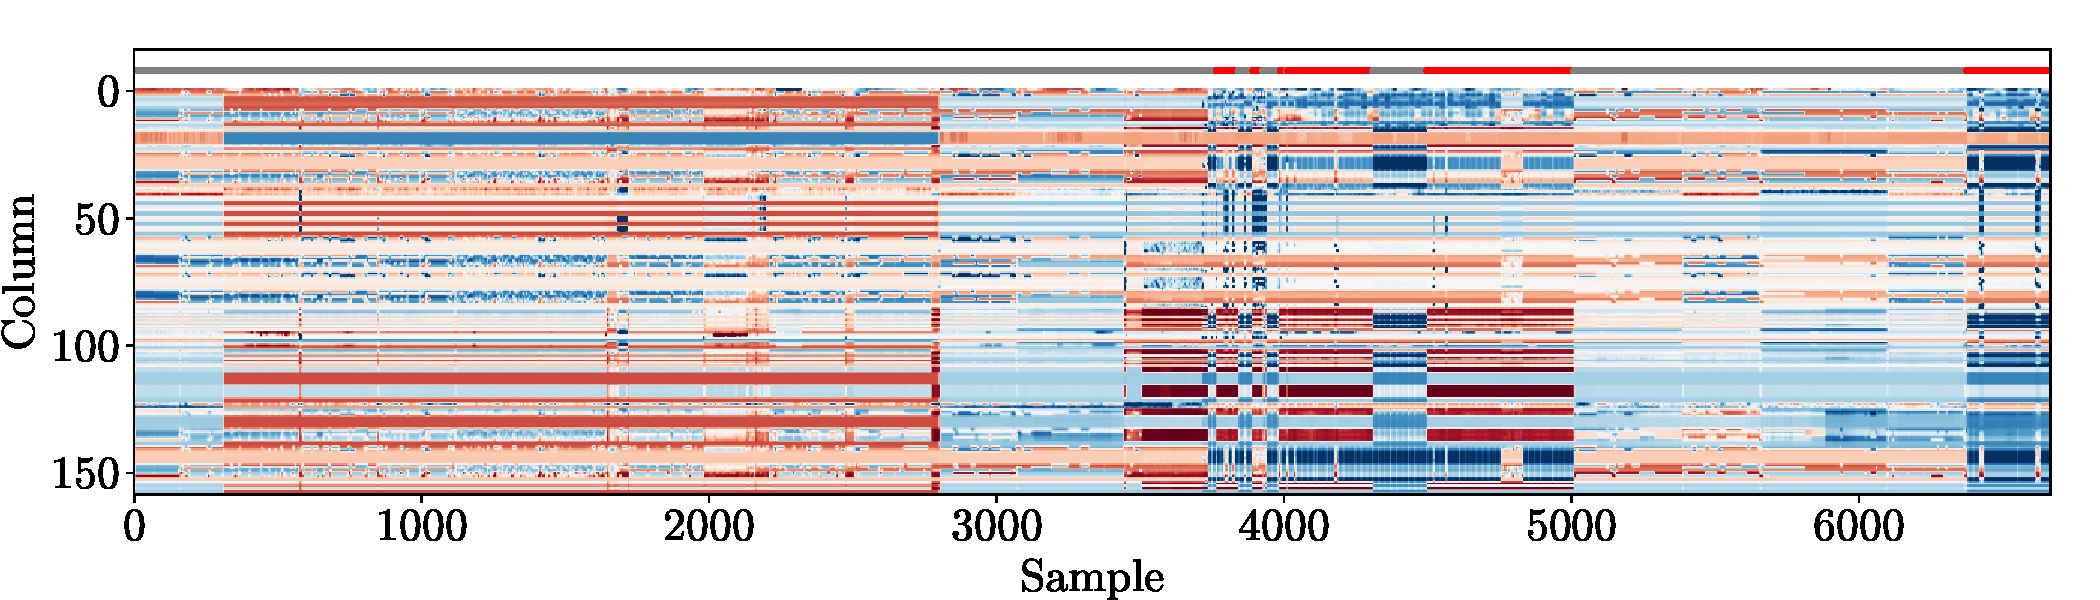
\includegraphics[width=0.9\linewidth]{./img/_ad_hpc_heatmap.pdf}
            \caption{
                \parbox[t]{0.75\linewidth}{Heatmap of the dataset. On the top line, gray points represent normal behavior while red points are anomalies. In the heatmap, white tiles represent the mean, red tiles represent values below average, and blue tiles represent values above average.}
            }
        \end{figure}
\end{description}



\section{Approaches}


\subsection{Multivariate KDE}

Given the train, validation, and test splits, the dataset is standardized using the training set alone. This avoids leaks from the test set.

The KDE model, bandwidth, and threshold are fitted as in \Cref{ch:ad_low}.

\begin{description}
    \item[Cost model]
        A simple cost model can be based on:
        \begin{itemize}
            \item False positives,
            \item False negatives,
            \item A time tolerance.
        \end{itemize}

    \item[Problems]
        KDE on this dataset has the following problems:
        \begin{itemize}
            \item It is highly subject to the curse of dimensionality and requires more data to be reliable.
            \item As the dataset is used during inference, a large dataset is computationally expensive.
            \item It only provides an alarm signal and not an explanation of the anomaly. In low-dimensionality, this is still acceptable, but with high-dimensional data it is harder to find an explanation.
        \end{itemize}
\end{description}